% !TEX root = ../pdf/stat205.tex
% [There are multiple stat205.tex files, but the one in ../pdf is the usual one]



%%%%%%%%%%%%%%%%%%%%%%%%%%%%%%%%%%%%%%%%%%%%%%%
\chapter{Probability Distributions}


\begin{verse}{\it
``When there are but two players, your theory which proceeds by combinations is very just. \\
But when there are three, I believe I have a proof that it is unjust that you should proceed in any other manner than the one I have.''\vspace*{6pt}} \\
\hspace*{2cm} -- Pascal's letter to Fermat\FOOTNOTE{from \url{https://www.york.ac.uk/depts/maths/histstat/pascal.pdf}}
\end{verse}
\vspace*{12pt}


\section{Random Variables}

In Example \autoref{exmp:three_fair_coins}, we denote the number of observed heads by \( X \),
which can take on values 0, 1, 2, or 3.
Each of these numbers corresponds to one of the following events:
\begin{itemize}
    \item 0: \( A = \{ TTT \} \),
    \item 1: \( B = \{ HTT, THT, TTH \} \),
    \item 2: \( C = \{ HHT, HTH, THH \} \),
    \item 3: \( D = \{ HHH \} \)
\end{itemize}
In other words, the sample space is partitioned into events \( A, B, C, \) and \( D \).
Hence, we can map each element of \( S \) to exactly one element of \( \{ 0, 1, 2, 3 \} \).
This mapping is achieved using \( X \), which is called a \keyterm{random variable}.

Thus:
\begin{gather*}
    X(TTT) = 0, X(HTT) = X(THT) = X(TTH) = 1, X(HHT) = X(HTH) = X(THH) = 2, X(HHH)= 3
\end{gather*}

More formally, in a probability model with sample space \( S \),
a random variable (or simply a variable) is a real-valued function \( X: S \rightarrow R \),
where the range of \( X \) is a subset of the real numbers.
The range of \( X \) is called the \keyterm{support} of \( X \) and is denoted by \( S_{X} \).

Conventionally, if \( A \subset R\), we define:
\begin{gather*}
    (X \in A) = \{ e \in S | X(e) \in A \}
\end{gather*}
For instance, in the previous example, \( (X < 2) = (X \in (-\infty, 2)) = (X \in \{ 0, 1 \}) = \{ TTT, HTT, THT, TTH \} \).

When working with random variables, probabilities can be expressed quantitatively.
For example, if we want the probability that the number of heads is fewer than 2, we are interested in the event \( (X < 2) \).
As shown earlier, this corresponds to:
\begin{gather*}
    P(X < 2) = P(X \in \{ TTT, HTT, THT, TTH \}) = \frac{4}{8} = \frac{1}{2}
\end{gather*}

\begin{exmp}
    Suppose in Example \autoref{exmp:heads_observe}, \( X \) is the number of coin tosses required to observe the first heads.
    Thus, the support of \( X \) is \( S_{X} = \{ 1, 2, \ldots \} \).
    For instance, if one iteration of this experiment yields the outcome \( TTTH \),
    then \( X(TTTH) = 4 \), as the first heads occurs on the fourth toss.

    The probability that the number of coin tosses required to observe the first heads is an odd number is given by:
    \begin{align*}
        P(X \in \{ 1, 3, \ldots \}) &= P(\{ H, TTH, \ldots \})\\
        &= P(\{ H \}) + P(\{ TTH \}) + \ldots\\
        &= (\frac{1}{2}) + (\frac{1}{2})^3 + \ldots\\
        &= \frac{2}{3}
    \end{align*}
\end{exmp}

\begin{exmp}
    In the previous example, what is the probability that more than six coin tosses are required to observe the first heads?
\end{exmp}

In the two examples we analyzed so far, the support \( S_{X} \) is countable.
In this case, we say \( X \) is a \keyterm{discrete random variable}.
Conversely, if a random variable can take on infinitely many (uncountable) number of values,
we call it a \keyterm{continuous random variable}.

Below are examples of continuous random variables:

\begin{exmp}
    In Example \autoref{exmp:lightbulb_lifespan}, let \( X \) be lightbulb's lifespan.
    Since lifespans can take any non-negative real value, \( X \) is a continuous random variable.
\end{exmp}

\begin{exmp}
    Suppose a needle is dropped at random into a circular disk of radius 3.
    The sample space consists of all possible landing positions of the needle, which are uncountable.
    Let \( X \) denote the distance from the needle's landing point to the center of the disk.
    Then \( X \) is a continuous random variable with support \( S_{X} = [0, 3] \),
    where the interval includes the boundary points (accounting for the possibility of landing exactly on the disk's edge).
\end{exmp}

\section{Probability Distribution}

We saw that different values of a random variable \( X \) implicitly partition the sample space into mutually exclusive events.
A key characteristic of any probability model is the probability it assigns to each possible value of the random variable.
When \( X \) is discrete (taking on countably many values), we can conveniently represent its \keyterm{probability distribution} using a graph, a table, or a function.
\begin{exmp}\label{exmp:three_dice_prob_dist}
    The probability distribution table for \( X \) (the number of observed heads) in Example \autoref{exmp:three_fair_coins} is:
	\begin{center}
	\begin{tabular}{|c|c|c|c|c|c|}
	\hline
	\( x \) & 0 & 1 & 2 & 3 & Total \\
	\hline
	\( P(X = x) \) & \( \frac{1}{8} \) & \( \frac{3}{8} \) & \( \frac{3}{8} \) & \( \frac{1}{8} \) & \( 1 \) \\
	\hline
	\end{tabular}
	\end{center}
    Note that the sum of all assigned probabilities equals 1, as expected.

    The corresponding graph is shown in \autoref{fig:three_dice_prob_dist}.
    \begin{figure}[t]
    \begin{center}
    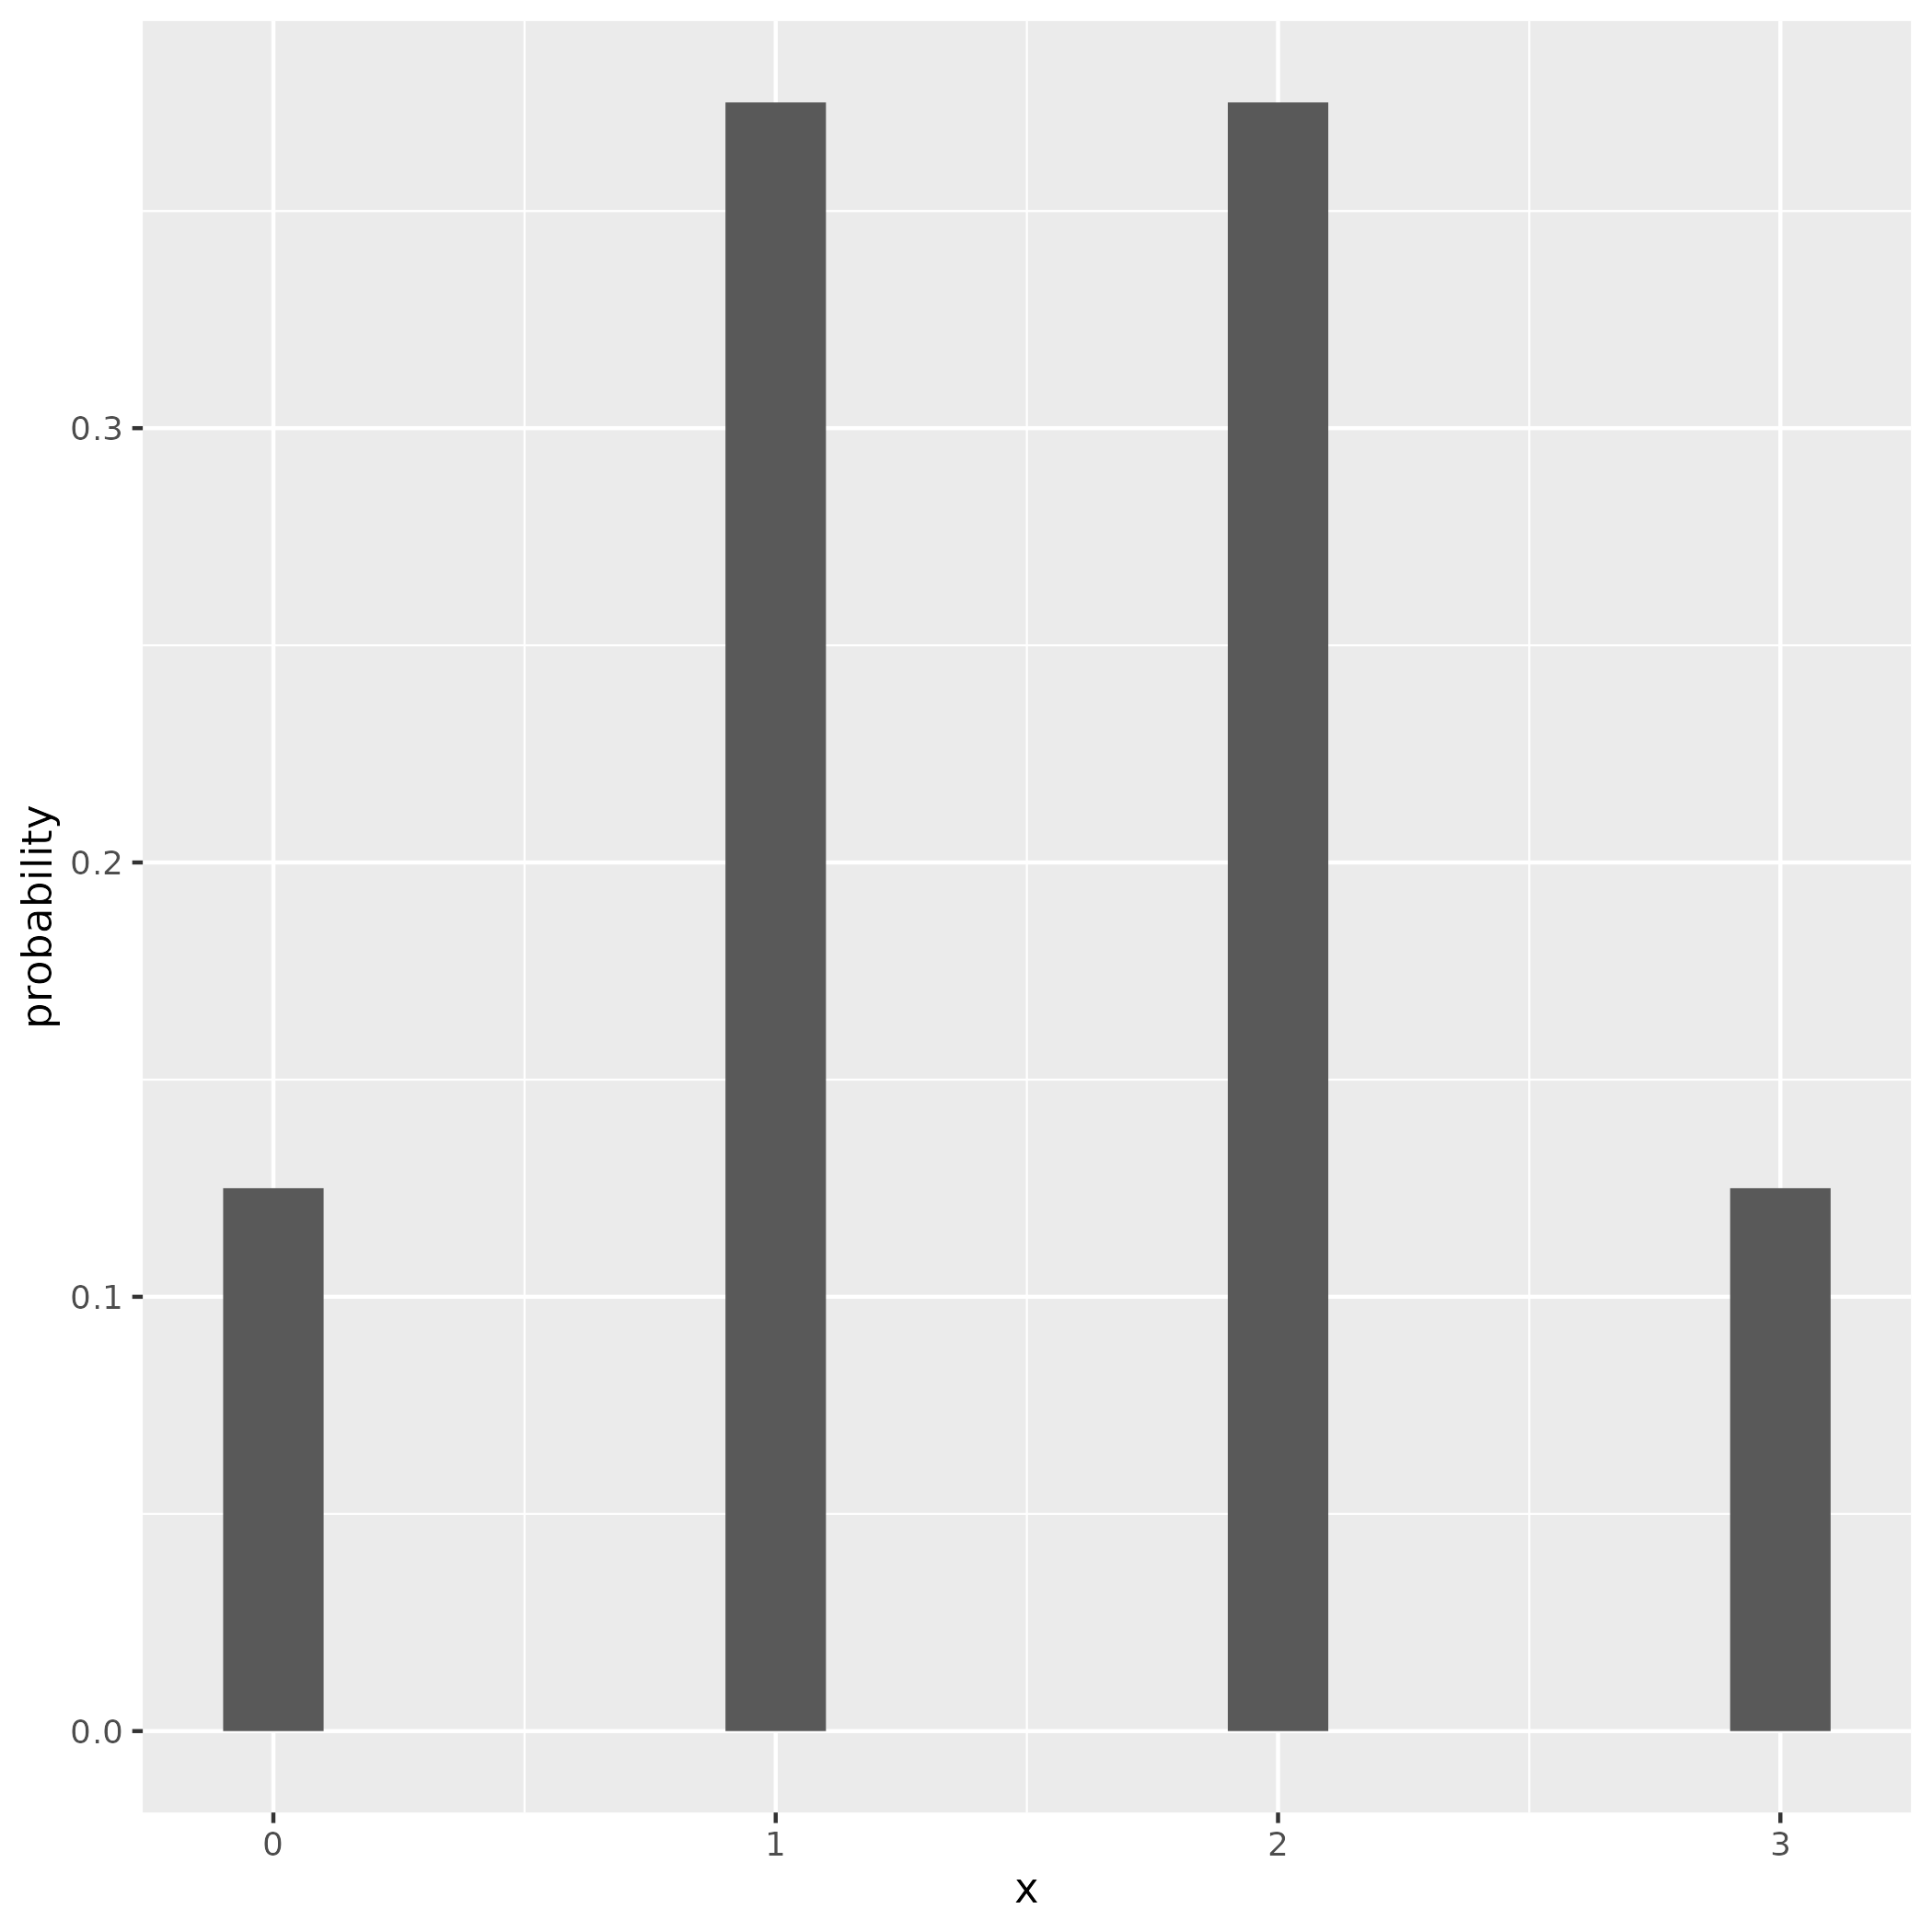
\epsfig{file=../img/threeDiceProbDistrib.png,clip=true,width=8.8cm}
    \end{center}
    \caption{Probability distribution graph for Example \autoref{exmp:three_dice_prob_dist}}
    \label{fig:three_dice_prob_dist}
    %\HR
    \end{figure}
\end{exmp}
For a discrete random variable \( X \), we can also describe its probability distribution using a function.
This function is called \keyterm{probability mass function (PMF)}, and is defined as follows:
\begin{align*}
    p_{X} \colon R &\to [0, 1] \\
    x &\mapsto P(X = x)
\end{align*}
where \( P \) is a probability measure.

All values of \( X \) without assigned probabilities are implicitly defined to be zero.
For instance, in the previous example, the PMF is:
\begin{gather*}
    p_{X}(x) = \begin{cases}
        \frac{1}{8}, & \text{if } x = 0, 3\\
        \frac{3}{8}, & \text{if } x = 1, 2\\
        0, & \text{O.W.}\\
    \end{cases}
\end{gather*}
Henceforth, when specifying a probability mass function (PMF), we will omit all values of the random variable that have zero probability.

\section{Discrete Distributions}

Many problems we encounter follow the same pattern in how they assign probabilities to different values of a random variable.
Here, we discuss two such cases for discrete random variables.

\subsection{Bernoulli Distribution}

In a coin toss, the outcome is either heads or tails (Example \autoref{exmp:coin_toss}).
When drawing a ball from an urn containing only blue and red balls, it's either red or blue.
When selecting a lamp from the box for quality inspection, each lamp is either functional or defective.

These are all examples of \keyterm{Bernoulli trial}, where an experiment yields exactly one of two possible outcomes.
We designate one outcome as a "success" (typically mapped to 1) and the other as a "failure" (mapped to 0).
The corresponding Bernoulli random variable \( X \) thus has the probability mass function:
\begin{gather*}
    p_{X}(x) = \begin{cases}
        p, & \text{if } x = 1\\
        1 - p, & \text{if } x = 0\\
    \end{cases}
    = p^x(1 - p)^{1 - x}
\end{gather*}
where \( x = 0, 1 \) and \( p \) is the probability of success.
We call \( X \) a \keyterm{Bernoulli random variable}, and we write \( X \sim Bern(p) \), indicating that X follows a \keyterm{Bernoulli distribution} with success probability \( p \).
\begin{exmp}
    Consider an unfair coin toss where the probability of landing heads is \( \frac{2}{3} \).
    Let \( X \) be the random variable representing the observation of heads. Then \( X \sim Bern(\frac{2}{3}) \).
\end{exmp}
\begin{exmp}
    For a fair six-sided die roll, let \( X \) be the indicator random variable for the event "not six."
    The success probability is observing 1, 2, 3, 4, or 5,
    which is \( p = \frac{5}{6} \),
    and thus \( X \sim Bern(\frac{5}{6}) \).
\end{exmp}

\subsection{Binomial Distribution}

Suppose \( n \) identical Bernoulli trials are performed independent of each other.
If \( X \) is the number of successes in these \( n \) trials, then it is called a \keyterm{binomial random variable}.
We say \( X \) follows a \keyterm{binomial distribution} and denote this by \( X \sim B(n, p) \),
where \( p \) is the probability of success and remains the same in each Bernoulli trial.

To compute the \( X \)'s PMF \( p_{X}(x) \),
we first choose \( x \) trials out of total \( n \) Bernoulli trials.
This can be done in \( n \choose x \) ways.
Now consider any one of these arrangements of \( x \) successes and \( n - x \) failures.
The following analysis focuses on the configuration depicted in \autoref{fig:binom_seq}.
\begin{figure}[t]
\begin{center}
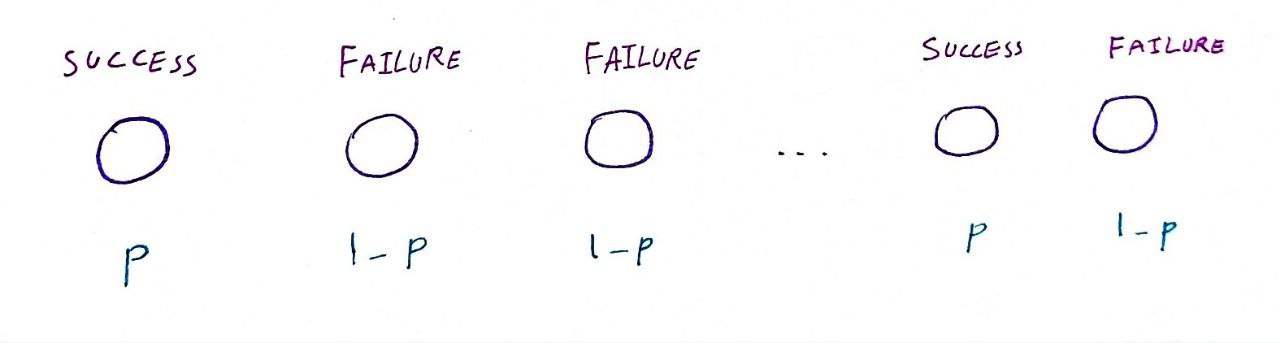
\epsfig{file=../img/binomSeq.jpg,clip=true,width=8.8cm}
\end{center}
\caption{one arrangement of \( x \) successes and \( n - x \) failures in \( n \) independent Bernoulli trials}
\label{fig:binom_seq}
%\HR
\end{figure}
What is the probability of such a sequence occurring?

Let \( S_i \) denote the event of success in the \( i \)-th trial and \( F_i \) the event of failure, where \( i = 1, 2, \ldots, n \).
Since the trials are independent of each other, the multiplication rule yields:
\begin{align*}
    P(S_1 \cap F_2 \cap F_3 \cap \ldots \cap S_{n - 1} \cap F_{n}) &= P(S_1)P(F_2)P(F_3)\ldots P(S_{n - 1})P(F_n)\\
    &= p(1 - p)(1 - p)\ldots p(1 - p)\\
    &= p^{x}(1 - p)^{n - x}
\end{align*}
Thus:
\begin{gather*}
    p_{X}(x) = \binom{n}{x} p^{x}(1 - p)^{n - x}
\end{gather*}
where \( x = 0, 1, 2, \ldots, n \).

We denoted the Bernoulli distribution by \( Bern(p) \) and the binomial distribution by \( B(n, p) \).
The values inside the parentheses define random variable's distribution and are called \keyterm{parameters}.
If we know these parameters, we can compute probabilities for each possible value.

Note that a binomial distribution with \( n = 1 \) is Bernoulli distribution.

\begin{exmp}
    A coin is tossed 8 times. What is the probability of observing 5 tails?
\end{exmp}
\begin{solution}
    Each coin toss is a Bernoulli trial where success is defined as observing trials.
    The probability of success is therefore \( p = \frac{1}{2} \).
    Let \( X \) be the number of tails in these 8 coin tosses.
    So \( X \sim B(8, \frac{1}{2}) \), and we can compute the desired probability:
    \begin{align*}
        p_{X}(5) &= \binom{8}{5} (\frac{1}{2})^5 (1 - \frac{1}{2})^{8 - 5}\\
        &= \frac{8 \times 7 \times 6 \times 5!}{3!5!} (\frac{1}{2})^8\\
        &= 56 \times \frac{1}{256}\\
        &\approx 0.21875
    \end{align*}
\end{solution}

\begin{exmp}
    In Example \autoref{exmp:three_dice_prob_dist}, \( X \sim B(3, \frac{1}{2}) \).
    So another way to find the probability distribution is:
    \begin{gather*}
        p_{X}(0) = \binom{3}{0} (\frac{1}{2})^0 (1 - \frac{1}{2})^{3 - 0} = 1 \times \frac{1}{8} = \frac{1}{8}\\
        p_{X}(1) = \binom{3}{1} (\frac{1}{2})^1 (1 - \frac{1}{2})^{3 - 1} = 3 \times \frac{1}{8} = \frac{3}{8}\\
        p_{X}(2) = \binom{3}{2} (\frac{1}{2})^2 (1 - \frac{1}{2})^{3 - 2} = 3 \times \frac{1}{8} = \frac{3}{8}\\
        p_{X}(3) = \binom{3}{3} (\frac{1}{2})^3 (1 - \frac{1}{2})^{3 - 3} = 1 \times \frac{1}{8} = \frac{1}{8}\\
    \end{gather*}
\end{exmp}
\begin{exmp}
    Based on a study, only 8\% of Canadians did not eat at restaurants last month.\FOOTNOTE{\url{https://www150.statcan.gc.ca/n1/pub/11-627-m/11-627-m2019003-eng.htm}}
    If you randomly survey 7 Canadians about their dining habits,
    what is the probability that exactly 3 of them ate out last month?
\end{exmp}
\begin{solution}
    Let \( X \) denote the number of individuals (out of 7 surveyed) who ate at restaurants last month.
    Since \( X \sim B(7, 0.92) \),
    \begin{gather*}
        p_{X}(3) = \binom{7}{3} (0.92)^3 (1 - 0.92)^{7 - 3} \approx 0.0011
    \end{gather*}
\end{solution}
For a random variable \( X \sim B(n, p) \), we can compute \( p_{X}(x) \) using this R command:
\begin{lstlisting}[language=R]
> dbinom(x, size, prob)
\end{lstlisting}
where \verb|x| is \( x \), \verb|size| is the number of trials \( n \), and \verb|prob| is the probability of success \( p \).

Following this approach, the previous example can be solved as follows:
\begin{lstlisting}[language=R]
> dbinom(3, 7, 0.92)
[1] 0.001116327
\end{lstlisting}
We can also find the probability distribution in Example \autoref{exmp:three_dice_prob_dist} in three commands:
\begin{lstlisting}[language=R]
> dbinom(0, 3, 0.5)
[1] 0.125
> dbinom(1, 3, 0.5)
[1] 0.375
> dbinom(2, 3, 0.5)
[1] 0.375
> dbinom(3, 3, 0.5)
[1] 0.125
\end{lstlisting}
or in a single command:
\begin{lstlisting}[language=R]
> dbinom(0:3, 3, 0.5)
[1] 0.125 0.375 0.375 0.125
\end{lstlisting}
Using \verb|sum()|, we can compute the total of outputs in the previous command, which equals 1 as expected:
\begin{lstlisting}[language=R]
> sum(dbinom(0:3, 3, 0.5))
[1] 1
\end{lstlisting}
\begin{exmp}\label{exmp:ucalgary}
    Suppose 11\% of University of Calgary graduates eventually pursue a PhD.
    If we randomly select 40 graduates,
    what is the probability that exactly 35 of them did not pursue (or will not pursue) doctoral studies?
    Calculate this probability by hand and using R.
\end{exmp}
\begin{solution}
    Let \( Y \) be the number of those who did not pursue (or will not pursue) doctoral studies.
    Therefore, \( Y \sim B(40, 0.89) \) with PMF:
    \begin{gather*}
        p_{Y}(y) = \binom{40}{y} 0.89^{y}0.11^{40 - y}
    \end{gather*}
    where \( y = 0, 1, 2, \ldots, 40 \).

    The desired probability is:
    \begin{gather*}
        p_{Y}(35) = \binom{40}{35} 0.89^{35}0.11^{40 - 35} \approx 0.18
    \end{gather*}
    The R command below verifies this result:
    \begin{lstlisting}[language=R]
> dbinom(35, 40, 0.89)
[1] 0.1794093
    \end{lstlisting}
\end{solution}
We may be interested in the left-tail probability \( P(X \leq q) \), where \( q \) can be any real number.
It is obvious that if \( q < 0 \), \( P(X \leq q) = 0 \), since \( X \) is defined for integers starting at zero.
However, for \( q \geq 0\), \( P(X \leq q) = p_{X}(0) + \ldots + p_{X}(\floor{q}) \).

In R, the following command computes this probability:
\begin{lstlisting}[language=R]
> pbinom(q, size, prob)
\end{lstlisting}
where \verb|q| is \( q \), \verb|size| is the number of trials \( n \), and \verb|prob| is the probability of success \( p \).

To compute \( P(X > q) \), set the optional parameter \verb|lower.tail| to \verb|FALSE|:
\begin{lstlisting}[language=R]
> pbinom(q, size, prob, lower.tail = FALSE)
\end{lstlisting}
which is equivalent to:
\begin{lstlisting}[language=R]
> 1 - pbinom(q, size, prob)
\end{lstlisting}
This is because \( P(X \in R) = 1 \) and \( R \) is partitioned into \( (-\infty, q] \) and \( (q, \infty) \).
Hence:
\begin{gather*}
    1 = P(X \in R) = P((X \leq q) \cup (X > q)) = P(X \leq q) + P(X > q)\\
    P(X > q) = 1 - P(X \leq q)
\end{gather*}
\begin{exmp}
    In Example \autoref{exmp:ucalgary}, the probability that at most 30 graduates did not pursue (or will not pursue) doctoral studies is:
    \begin{lstlisting}[language=R]
> pbinom(30, size = 40, prob = 0.89)
[1] 0.009816241
    \end{lstlisting}
    While the probability that more than 30 of them did not pursue (or will not pursue) doctoral studies is:
    \begin{lstlisting}[language=R]
> pbinom(30, size = 40, prob = 0.89, lower.tail = FALSE)
[1] 0.9901838
    \end{lstlisting}
    since \( P(Y > 30) = P(Y \geq 31) \).
    This also equals \( p_{Y}(31) + p_{Y}(32) + \ldots + p_{Y}(40) \):
    \begin{lstlisting}[language=R]
> sum(dbinom(31:40, size = 40, prob = 0.89))
[1] 0.9901838
    \end{lstlisting}
    The probability that between 10 and 35 (inclusive) of the selected graduates did not pursue (or will not pursue) doctoral studies is:
    \begin{lstlisting}[language=R]
> sum(dbinom(10:35, size = 40, prob = 0.89))
[1] 0.4532124
    \end{lstlisting}
    or using \verb|pbinom()|:
    \begin{lstlisting}[language=R]
> pbinom(35, size = 40, prob = 0.89) - pbinom(9, size = 40, prob = 0.89)
[1] 0.4532124
    \end{lstlisting}
    since:
    \begin{align*}
        P(Y \leq 35) - P(Y \leq 9) &= \sum_{i = 0}^{35} p_{Y}(i) - \sum_{j = 0}^{9} p_{Y}(j)\\
        &= p_{Y}(10) + p_{Y}(11) + \ldots + p_{Y}(35)
    \end{align*}
\end{exmp}

\section{Continuous Distributions}

We now discuss two examples of continuous random variables.
We defined the concept of probability mass function for discrete random variables,
which assigned a probability for each possible value of the random variable.
One way to conceptualize this is as the distribution of a unit mass across a countable set of discrete points.
Even when there are an infinite number of these points,
it is possible to assign probabilities so that their sum equals 1.
For instance, let \( X \) be a random variable with support \( S_{X} = \{ 1, 2, 3, \ldots \} \).
Defining the PMF to be \( p_{X}(x) = \frac{1}{2^x} \),
it can be easily shown that this is a valid PMF.\FOOTNOTE{see the Wikipedia page on \href{https://en.wikipedia.org/wiki/1/2_\%2B_1/4_\%2B_1/8_\%2B_1/16_\%2B_\%E2\%8B\%AF}{the series \( \frac{1}{2} + \frac{1}{4} + \frac{1}{8} + \cdots \)}}

However, continuous random variables can take on uncountably many values,
making it impossible to assign positive probability to each single point.
This time, instead of a countable number of points, consider a unit-mass rod (which could be finite, infinite, or a combination of rods). 
Unlike discrete distributions where mass concentrates at points, here we only discuss mass contained within intervals.
Just as a perfectly thin cross-section of a rod contains no mass, continuous distributions assign zero probability to single points.
Only interval-based measurements yield non-zero values.

You can again interpret the probability distribution as a unit mass distribution.
Following this analogy, for a continuous random variable \( X \),
we have \( P(X = x) = 0 \) at every point \( x \in S_{X} \).

To better understand the continuous distributions, we start with a simple and basic one.

\subsection{Continuous Uniform Distribution}

Suppose the unit mass is uniformly distributed on the interval \( S_{X} = [a, b] \).
This is analogous to a rod of length \( b - a \) with uniform density.
The rod's linear density is therefore \( \frac{1}{b - a} \),
which we call \keyterm{probability density function (PDF)} and denote it by \( f_{X}(x) = \frac{1}{b - a} \).
We say that \( X \) follows a \keyterm{continuous uniform distribution} over the interval \( [a, b] \), denoted \( X \sim U(a, b) \).

Here, the PDF is independent of \( x \), since the unit mass is distributed uniformly.
\autoref{fig:uniform_graph} shows the corresponding graph.
The area under the uniform density function equals 1, representing total probability mass.
Also, for any interval \( [c, d] \subset [a, b] \),
the probability \( P(c \leq X \leq d) \) corresponds to the area under the probability density function (PDF) over this interval,
which in this case is calculated as \( (d - c) \times \frac{1}{b - a} \).
\begin{figure}[t]
\begin{center}
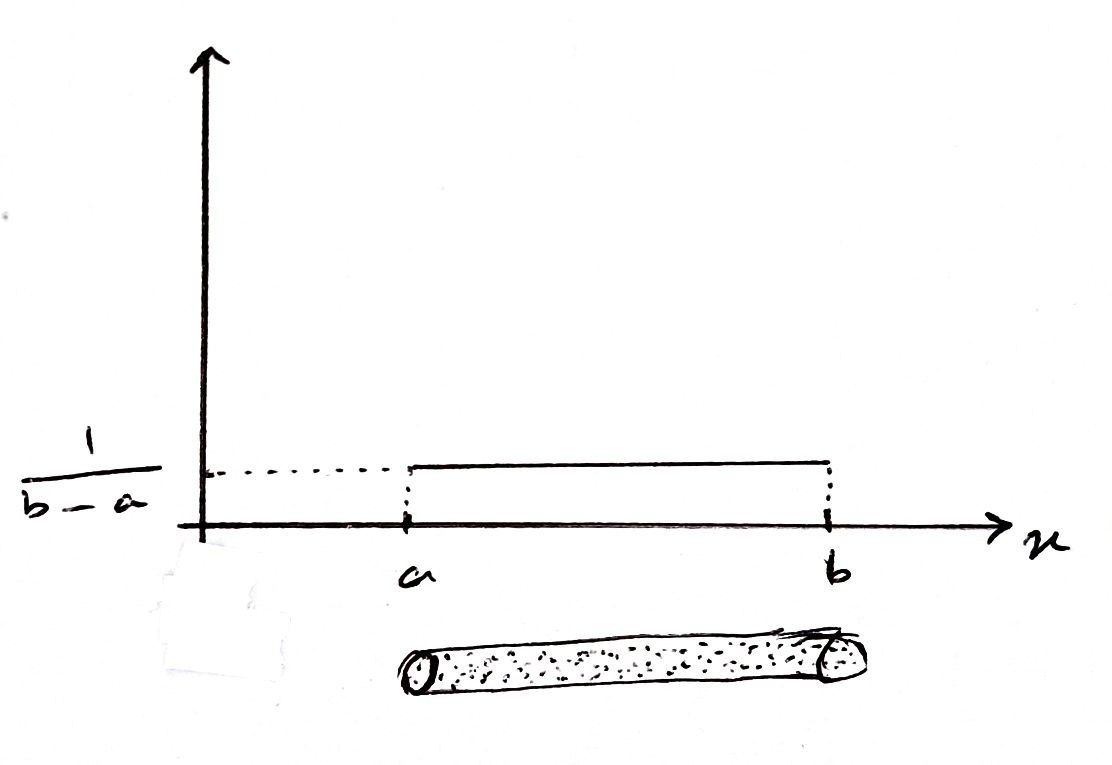
\epsfig{file=../img/uniformGraphWithRod.jpg,clip=true,width=8.8cm}
\end{center}
\caption{uniform distribution graph with unit-mass rod analogy}
\label{fig:uniform_graph}
%\HR
\end{figure}

\begin{exmp}
    A number is selected randomly between 3 and 7 (inclusive).
    \begin{enumerate}
        \item What is the probability that it equals 3.4?
        \item What is the probability that it lies between 4 and 6 (inclusive)?
    \end{enumerate}
\end{exmp}
\begin{solution}
    Let X be the selected number.
    Then \( X \sim U(3, 7) \),
    and the PDF is \( f_{X}(x) = \frac{1}{7 - 3} = \frac{1}{4} \) where \( 3 \leq x \leq 7 \).
    \begin{enumerate}
        \item \( P(X = 3.4) = 0 \)
        \item \( P(4 \leq X \leq 6) = (6 - 4) \times \frac{1}{4} = 0.5 \)
    \end{enumerate}
\end{solution}

\subsection{Normal (Gaussian) Distribution}

The PDF of a \keyterm{normal random variable} \( X \) is:
\begin{gather*}
    f_{X}(x) = \frac{1}{\sigma\sqrt{2\pi}}e^{-\frac{1}{2}(\frac{x - \mu}{\sigma})^2}
\end{gather*}
where \( x, \mu \in R \) and \( \sigma > 0 \).
\( \mu \) and \( \sigma \) are parameters of this distribution.
We say \( X \) is \keyterm{normally distributed} and denote it by \( X \sim N(\mu, \sigma) \).

The probability density function (PDF) of a normal distribution forms a symmetric bell-shaped curve, as illustrated in \autoref{fig:normal_graph}.
\begin{figure}[t]
\begin{center}
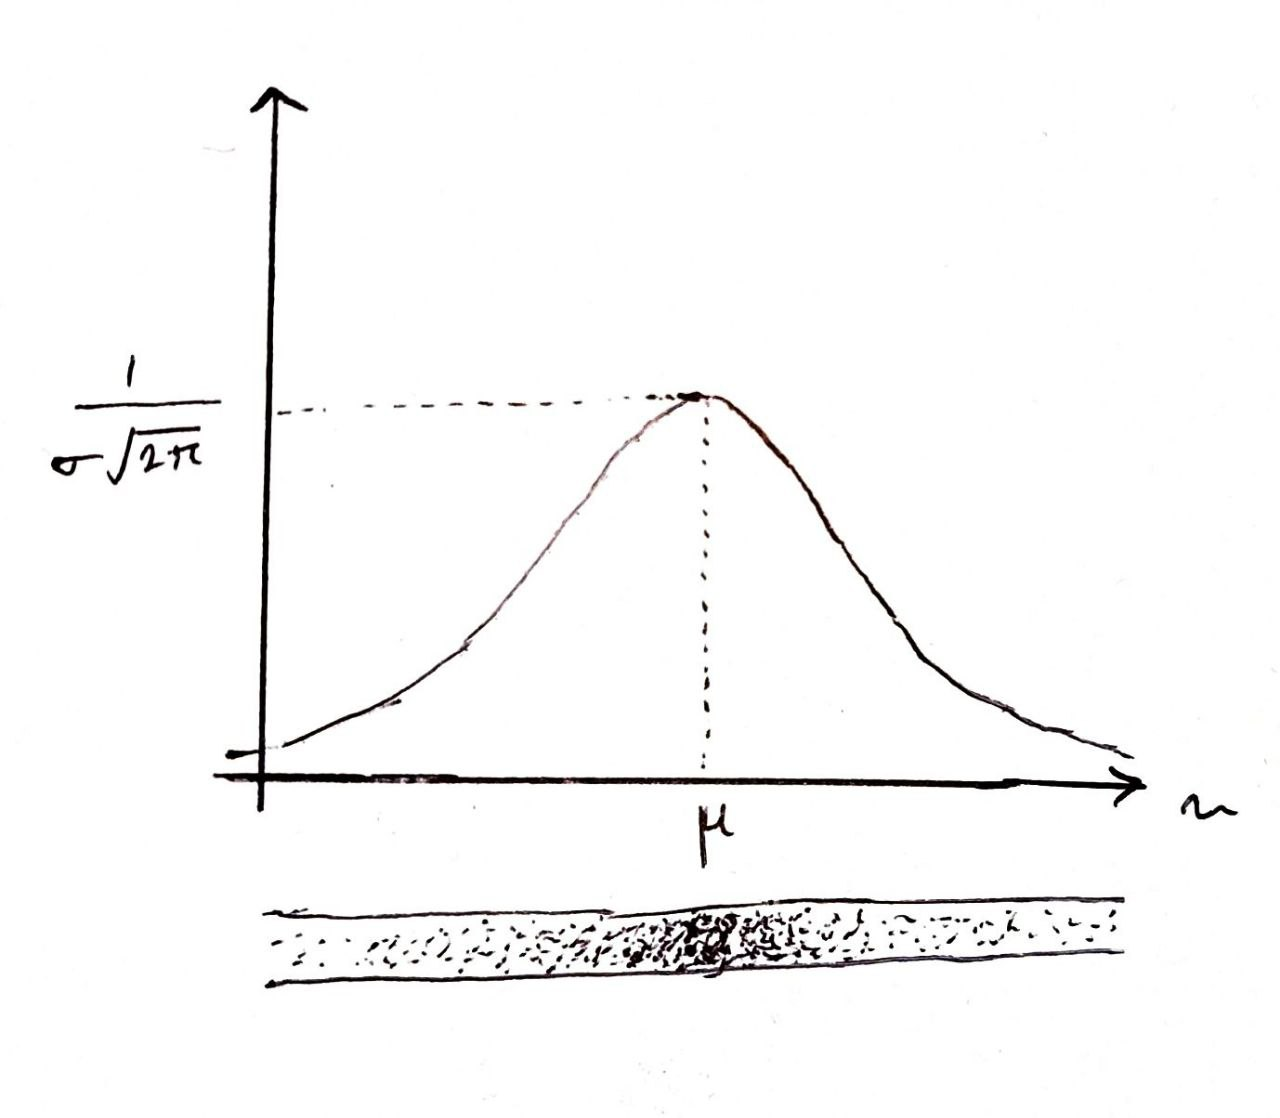
\epsfig{file=../img/normalGraphWithRod.jpg,clip=true,width=8.8cm}
\end{center}
\caption{normal distribution graph with unit-mass rod analogy}
\label{fig:normal_graph}
%\HR
\end{figure}
Unlike continuous uniform distribution, normal PDF depends on \( x \).
As we can see from this graph, most of the probability mass is concentrated around \( x = \mu \).
The density decreases as we move away from this point in either direction.

Many of the natural phenomena follow this pattern.
Grades of students of a class peak at an average grade, like 3.0, and it is less common for students to have high grades like 4.0 or low grades like 1.0.
The average height for men is approximately 5'7"\FOOTNOTE{from \url{https://www.verywellhealth.com/average-height-for-men-8421400}},
with heights becoming increasingly less probable as they deviate further from this number in either direction.

Similar to continuous uniform distribution, the area under the PDF represents total probability mass which equals 1.
Since the curve is symmetric around \( \mu \), \( P(X < \mu) = P(X > \mu) = 0.5 \).

The parameters \( \mu \) and \( \sigma \) are called \keyterm{location parameter} and \keyterm{scale parameter} respectively.
The location parameter determines the location of normal PDF's peak, while the scale parameter controls the dispersion of the PDF.
\autoref{fig:varying_normal_parameters} demonstrates the effects of varying the location parameter (\( \mu \)) and scale parameter (\( \sigma \)) independently while holding the other constant.
\FOOTNOTE{the visualizations were generated using the normal distribution tool at: \url{https://www.acsu.buffalo.edu/~adamcunn/probability/normal.html}}
\begin{figure}[t]
\begin{center}
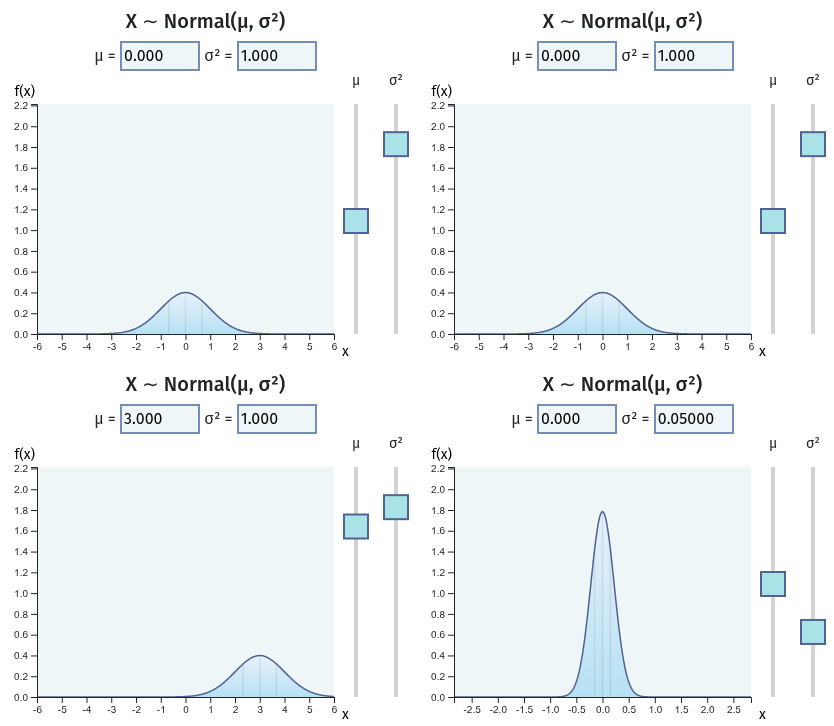
\epsfig{file=../img/varyingNormalParameters.png,clip=true,width=10cm}
\end{center}
\caption{Top-to-bottom: \( \mu \) increases cause rightward translation; \( \sigma \) decreases cause horizontal contraction.}
\label{fig:varying_normal_parameters}
%\HR
\end{figure}
For binomial random variables, we could compute probabilities at specific points using R's \verb|dbinom| function.
However, for a normal random variable \( X \sim N(\mu, \sigma) \),
\verb|dnorm| evaluates the probability density function (PDF) at any point:
\begin{lstlisting}[language=R]
> dnorm(x, mean, sd)
\end{lstlisting}
where \verb|x| is \( x \), \verb|mean| is the mean parameter \( \mu \), and \verb|sd| is standard deviation \( \sigma \).

Similar to \verb|pbinom|, the command \verb|pnorm| computes the probability \( P(X \leq q) \):
\begin{lstlisting}[language=R]
> pnorm(q, mean, sd)
\end{lstlisting}
where \verb|q| is \( q \), \verb|mean| is the mean parameter \( \mu \), and \verb|sd| is standard deviation \( \sigma \).
The output equals the area under the normal PDF to the left of \( q \) (see \autoref{fig:normal_lower_probability}).
\begin{figure}[t]
\begin{center}
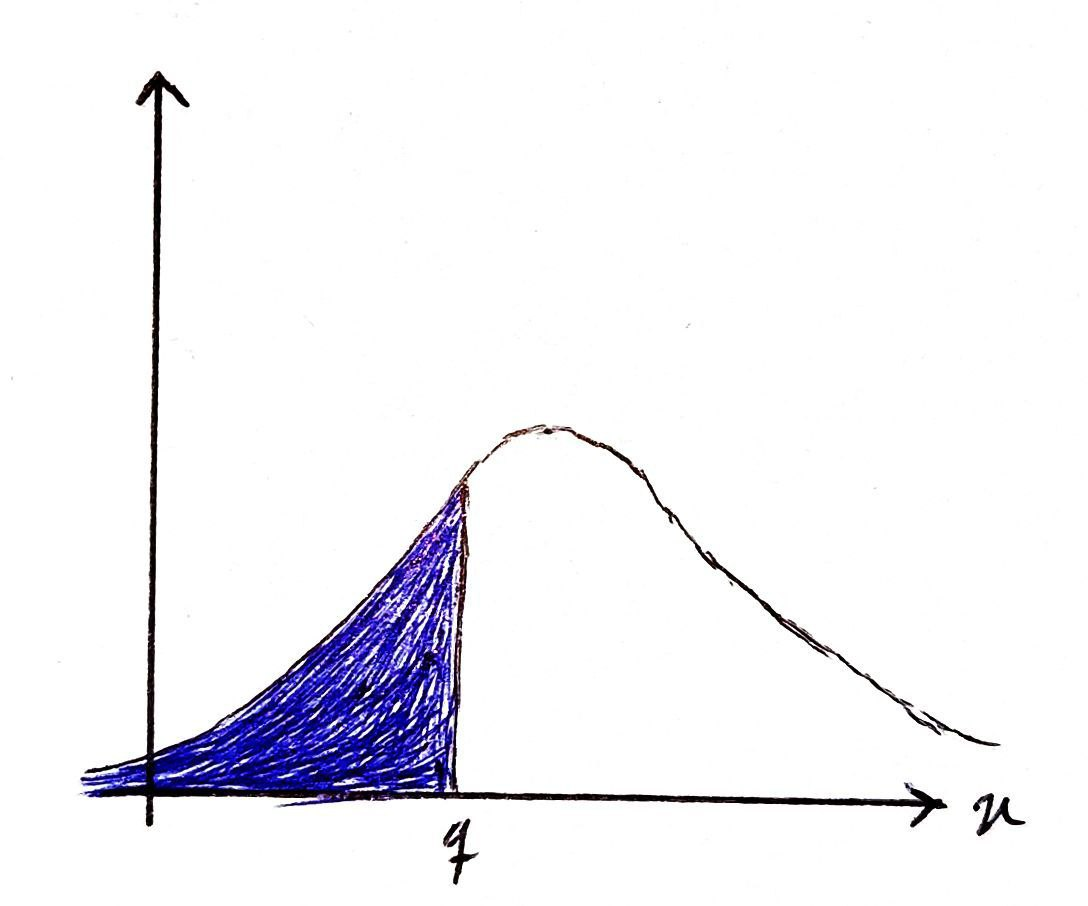
\epsfig{file=../img/normalLowerProbability.jpg,clip=true,width=10cm}
\end{center}
\caption{the blue-shaded area is \( P(X \leq q) \)}
\label{fig:normal_lower_probability}
%\HR
\end{figure}

We can use \verb|lower.tail = FALSE| to compute \( P(X > q) \):
\begin{lstlisting}[language=R]
> pnorm(q, mean, sd, lower.tail = FALSE)
\end{lstlisting}

\begin{exmp}\label{exmp:women_heights}
    The heights of women in a city follows a normal distribution with an average height of 165 cm and a standard deviation of 5 cm.
    \begin{enumerate}
        \item What is the probability that a woman's height is less than 170 cm?
        \item What is the probability that a woman's height is between 170 and 180 cm?
    \end{enumerate}
\end{exmp}
\begin{solution}
    Suppose a woman is chosen at random from this city.
    Let \( X \) denote her height.
    Thus, \( X \sim N(165, 5) \).
    \begin{enumerate}
        \item The desired probability is \( P(X < 170) \), but note that this is the same as \( P(X \leq 170) \).
        In other words, the probability is the area under the curve of this normal PDF over the interval \( (-\infty, 170) \),
        and the endpoint 170 itself contributes no probability mass.
        Therefore, we can equivalently compute the probability over the interval \( (-\infty, 170] \).

        Using R, we calculate:
        \begin{lstlisting}[language=R]
> pnorm(170, mean = 165, sd = 5)
[1] 0.8413447
        \end{lstlisting}
        \item The desired probability mass lies on the interval \( (170, 180) \).
        Note that inclusivity or exclusivity doesn't matter since we are dealing with a continuous probability distribution.

        This desired probability is:
        \begin{align*}
            P(170 < X < 180) &= P(X < 180) - P(X \leq 170)\\
            &= P(X \leq 180) - P(X \leq 170)
        \end{align*}
        which equals:
        \begin{lstlisting}[language=R]
> pnorm(180, mean = 165, sd = 5) - pnorm(170, mean = 165, sd = 5)
[1] 0.1573054
        \end{lstlisting}
        This is equivalent to removing the probability mass concentrated on the interval \( (-\infty, 170] \) from the probability mass concentrated on the interval \( (-\infty, 180) \).
    \end{enumerate}
\end{solution}
Now suppose that we want to find \( x_0 \) such that \( P(X \leq x_0) = p \) where \( p \in [0, 1] \).
The value of \( x_0 \) is the \( 100p \)th percentile of the distribution.
The following R command computes the value of \( x_0 \):
\begin{lstlisting}[language=R]
> qnorm(p, mean, sd)
\end{lstlisting}
where \verb|p| is the left-tail probability  \( p \), \verb|mean| is the mean parameter \( \mu \), and \verb|sd| is standard deviation \( \sigma \).
\begin{exmp}
    As we saw in \autoref{fig:normal_graph}, 50\% of the total probability mass lies in the interval \( (-\infty, \mu) \), where \( mu \) is the mean of the normal distribution.
    So we expect \verb|qnorm(0.5, mean, sd)| to return \verb|mean|, regardless of the standard deviation \verb|sd|.
    We can check this for some values:
    \begin{lstlisting}[language=R]
> qnorm(0.5, mean = 40, sd = 5)
[1] 40
> qnorm(0.5, mean = 40, sd = 10)
[1] 40
> qnorm(0.5, mean = 50, sd = 10)
[1] 50
> qnorm(0.5, mean = 50, sd = 5)
[1] 50
    \end{lstlisting}
    The default parameters for \verb|mean| and \verb|sd| are 0 and 1, respectively. Thus:
    \begin{lstlisting}[language=R]
> qnorm(0.5)
[1] 0
    \end{lstlisting}
\end{exmp}
\begin{exmp}
    In Example \autoref{exmp:women_heights}, what is the 80th percentile height?
\end{exmp}
\begin{solution}
    We compute \( x_0 \) such that \( P(X \leq x_0) = 0.8 \):
    \begin{lstlisting}[language=R]
> qnorm(0.8, mean = 165, sd = 5)
[1] 169.2081        
    \end{lstlisting}
\end{solution}

\subsection{Standard Normal Distribution}

Suppose Ellie purchased one watch from Henry for \$170 and another from Richard for \$180.
Henry watch sales follow a normal distribution with mean \$160 and standard deviation \$40,
while Richard's follow a normal distribution with mean \$190 and standard deviation \$20.
The question is: Which seller offered the better price?

The two watch prices follow different normal distributions, making direct price comparisons invalid.
However, any normally distributed random variable \( X \sim N(\mu, \sigma) \) can be converted to a \keyterm{standard normal random variable} \( Z \sim N(0, 1) \).
It can be proven that if \( X \sim N(\mu, \sigma) \), then defining \( Z = \frac{X - \mu}{\sigma} \) yields \( Z \sim N(0, 1) \).

In the example above, let \( X \) represent Henry's watch prices and \( Y \) represent Richard's watch prices.
Note that as \( X \) and \( Y \) are random variables, it is incorrect to state \( X = \$170 \) or \( Y = \$180 \).
Rather, \$170 represents a realization of \( X \) and \$180 a realization of \( Y \), and we denote them by \( x \) and \( y \), respectively.
Since \( \frac{X - 160}{40} \sim N(0, 1) \) and \( \frac{Y - 190}{20} \sim N(0, 1) \), both \( z_1 = \frac{x - 160}{40} = 0.25 \) and \( z_2 = \frac{y - 190}{20} = -0.5 \) can be thought of as realizations of the same normal distribution with mean 0 and standard deviation 1.
In other words, it is as if Ellie has purchased both watches from a single seller whose sells has a normal distribution with mean \$0 and standard deviation \$1.
\( z_1 \) and \( z_2 \) are called the \keyterm{standardized scores} or \keyterm{z-scores} of \( x \) and \( y \), respectively.

For any constant \( k \), when \( x = \mu + k\sigma \), the corresponding z-score is:
\begin{gather*}
    z = \frac{(\mu + k\sigma) - \mu}{\sigma} = k
\end{gather*}
Conversely, a z-score of \( k \) implies that the original value lies \( |k| \) standard deviations above the original mean if \( k > 0 \) and \( |k| \) standard deviations below the original mean if \( k < 0 \).

Returning to our example, \( z_1 = 0.25 \) means the price of the watch bought from Henry is 0.25 standard deviations above \$160, the average price at which Henry sells his watches,
while \( z_2 = -0.5 \) means the price of the watch bought from Richard is 0.5 standard deviations below \$190, the average price at which Richard sells his watches.
While Henry's price initially appears better, Richard actually sold the watch below his average price!

Converting a normal variable to standard variable is called \keyterm{standardization}, and can be used for such comparisons.

\begin{exmp}
    \begin{enumerate}
        \item Find \( P(Z < 1.4) \).
        \item \( P(Z > z_0) = 0.75 \). Find \( z_0 \).
        \item \( P(1 < Z < z_0) = 0.15 \). Find \( z_0 \).
    \end{enumerate}
\end{exmp}
\begin{solution}
    \begin{enumerate}
        \item Because \( Z \sim N(0, 1) \), we can compute the probability using:
    \begin{lstlisting}[language=R]
> pnorm(1.4, mean = 0, sd = 1)
[1] 0.9192433      
    \end{lstlisting}
    However, we saw that the default parameters for \verb|pnorm()| are already set to \verb|mean = 0| and \verb|sd = 1|.
    Therefore, the parameters can be omitted:
    \begin{lstlisting}[language=R]
> pnorm(1.4)
[1] 0.9192433      
    \end{lstlisting}
    \item We can use \verb|qnorm()| with the parameter \verb|lower.tail| set to \verb|TRUE|:
    \begin{lstlisting}[language=R]
> qnorm(0.75, mean = 0, sd = 1, lower.tail = FALSE)
[1] -0.6744898
    \end{lstlisting}
    or equivalently:
    \begin{lstlisting}[language=R]
> qnorm(0.75, lower.tail = FALSE)
[1] -0.6744898
    \end{lstlisting}
    Using the probability identity from the previous section \( P(Z > z_0) = 1 - P(Z \leq z_0) \), we obtain:
    \begin{gather*}
        P(Z \leq z_0) = 1 - P(Z > z_0) = 1 - 0.75 = 0.25\\
        P(Z \leq z_0) = 0.25
    \end{gather*}
    Thus, alternatively, we can use this command to find \( z_0 \) such that \( P(Z \leq z_0) = 0.25 \):
    \begin{lstlisting}[language=R]
> qnorm(0.25)
[1] -0.6744898
    \end{lstlisting}
    \item We have:
    \begin{align*}
        P(1 < Z < z_0) &= P(Z < z_0) - P(Z \leq 1)\\
        &= P(Z \leq z_0) - P(Z \leq 1)
    \end{align*}
    This yields:
    \begin{align*}
        P(Z < z_0) &= P(1 < Z < z_0) + P(Z \leq 1)\\
        &= 0.15 + P(Z \leq 1)
    \end{align*}
    Thus, \( z_0 \) equals:
    \begin{lstlisting}[language=R]
> qnorm(0.15 + pnorm(1))
[1] 2.380045
    \end{lstlisting}
    \end{enumerate}
\end{solution}

\section{Empirical Rule}

The \keyterm{Empirical Rule} (or \keyterm{68-95-99.7 Rule}) quantifies how probability mass concentrates within successive standard deviations of the mean in a normal distribution \( N(\mu, \sigma) \).
Specifically:
\begin{itemize}
    \item approximately 68\% of the probability mass lies within one standard deviation of the mean:
    \begin{lstlisting}[language=R]
> pnorm(1) - pnorm(-1)
[1] 0.6826895      
    \end{lstlisting}
    \item approximately 95\% of the probability mass lies within two standard deviations of the mean:
    \begin{lstlisting}[language=R]
> pnorm(2) - pnorm(-2)
[1] 0.9544997
    \end{lstlisting}
    \item approximately 99.7\% of the probability mass lies within three standard deviations of the mean:
    \begin{lstlisting}[language=R]
> pnorm(3) - pnorm(-3)
[1] 0.9973002
    \end{lstlisting}
\end{itemize}
We will examine practical applications of this rule in later chapters.
When modeling data using a normal distribution approximation with mean \( \mu \) and standard deviation \( \sigma \),
observations falling outside \( [\mu - 3\sigma, \mu + 3\sigma] \) are generally considered outliers.
This follows from the concentration of approximately 99.7\% of the probability mass within this interval,
leaving only 0.3\% of expected observations in the tails.
An illustration of this rule can be found at \href{https://andymath.com/normal-distribution-empirical-rule/}{this link}.

\begin{exmp}
    Let \( X \) represent the height (in cm) of a woman in the city from Example \autoref{exmp:women_heights}.
    \begin{enumerate}
        \item For a randomly selected woman with height 185 cm, compute her standardized height.
        \item Would you say that this woman is unusually tall?
    \end{enumerate}
\end{exmp}
\begin{solution}
    Let \( x \) be the height of this woman.
    \begin{enumerate}
        \item \begin{gather*}
            z = \frac{x - \mu}{\sigma} = \frac{185 - 165}{5} = 4
        \end{gather*}
        \item The computed z-score reveals that her height is four standard deviations above the city's mean.
        Since we defined outliers as data points beyond three standard deviations from the mean,
        this woman's height is undoubtedly an outlier!
    \end{enumerate}
\end{solution}

\section{Sampling Distribution and Central Limit Theorem}

This section introduces the Central Limit Theorem (CLT).
First developed by de Moivre (1733) for Bernoulli trials,
the theorem was subsequently generalized by Laplace, Cauchy, and others,
reaching its modern form in the early 20th century.

\subsection{Random Sample}

Let \( X \) be a random variable representing, for example, heights in a population, student IQ scores, daily milk consumption, etc.
A \keyterm{random sample} from this distribution consists of \( n \) independent and identically distributed (i.i.d.) random variables, each with the same distribution as \( X \).
Suppose, for instance, \( X \) represents the leaf lengths (in cm) of individuals in a specific plant species, where \( X \sim N(10, 2) \).
A random sample from this distribution consists of \( n \) independent observations \( X_1, X_2, \ldots, X_n \), each drawn from \( N(10, 2) \).
In other words, it's like randomly selecting \( n \) individual plans from our studied species and measuring their leaf lengths.
For a sample size of \( n = 4 \), we might obtain measurements like \( x_1 = 5, x_2 = 10.5, x_3 = 12.4, x_4 = 4.6 \),
or \( x_1 = 3.8, x_2 = 11, x_3 = 7.3, x_4 = 9 \).
Note that we denote random variables by uppercase letters (e.g., \( X, Y \)) and their observed values by corresponding lowercase letters (e.g., \( x, y \)).

\subsection{The Central Limit Theorem}

Consider a population of five individuals with ages 27, 31, 35, 28, and 33 years.
Let \( X \) represent an individual's age from this population.
The average age is therefore \( \mu = \frac{27 + 31 + 35 + 28 + 33}{5} = 30.8 \).
We now examine all possible random samples of size 4 that can be drawn from this population.

From multiplication principle, there are \( 5 \times 4 \times 3 \times 2 = 120 \) possible ordered samples \( x_1, x_2, x_3, x_4 \) when sampling without replacement (i.e., when each selected individual is removed from the population after selection, so no repeats can occur in an observed sample).

What we are interested in, however, is each sample's mean.
Since the ordering is irrelevant, we need only consider \( 5 \choose 4 \) distinct samples.
The table below displays these samples, which is called \keyterm{the sampling distribution of the sample mean}:
\begin{center}
\begin{tabular}{|c|c|c|}
\hline
\textbf{Sample} & \textbf{Sample Values} & \textbf{Sample Mean} \\ 
\hline
1 & 27, 31, 35, 28 & 30.25 \\
\hline
2 & 27, 31, 35, 33 & 31.5 \\
\hline
3 & 31, 35, 28, 33 & 31.75 \\
\hline
4 & 27, 35, 28, 33 & 30.75 \\
\hline
5 & 27, 31, 28, 33 & 29.75 \\
\hline
\end{tabular}
\end{center}
This yields that the average of all sample means is \( \mu_{\bar{X}} = \frac{30.25 + 31.5 + 31.75 + 30.75 + 29.75}{5} = 30.8 \),
which equals the population mean \( \mu \).

The distribution of sample means is illustrated in \autoref{fig:sample_means_alt}.
This figure demonstrates that the distribution of sample means approximates a normal distribution,
with the highest observed sample mean at 31.75 and values decreasing toward both tails.
\begin{figure}[t]
\begin{center}
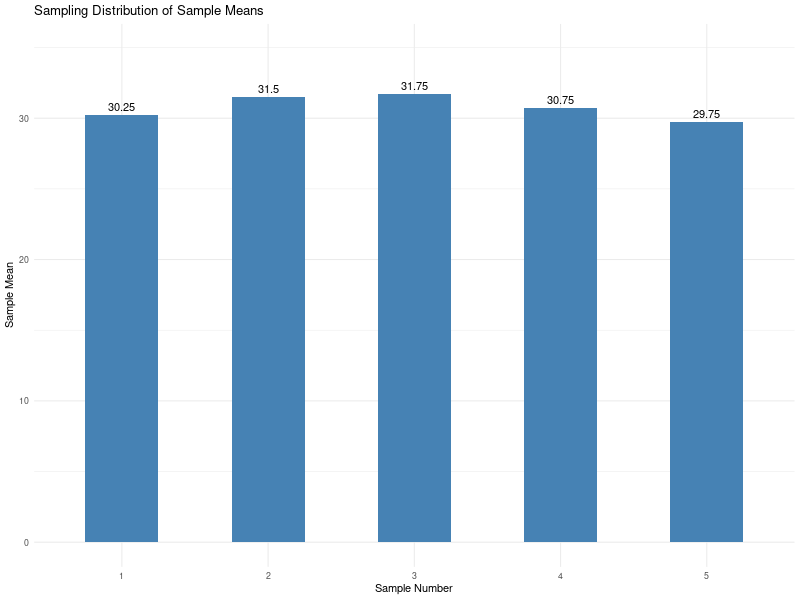
\epsfig{file=../img/sample_means_alt.png,clip=true,width=15cm}
\end{center}
\caption{sampling distribution of sample means}
\label{fig:sample_means_alt}
%\HR
\end{figure}

This is due to an important theorem in probability, known as \keyterm{the Central Limit Theorem (CLT)}.
Consider a random sample \( X_1, X_2, \ldots, X_n \) drawn from a population with \textit{arbitrary} distribution, mean \( \mu \), and \textit{finite} standard deviation \( \sigma \).
This theorem states that for sufficiently large \( n \) (typically at least 25 or 30 in practice), \( \bar{X} \sim N(\mu, \frac{\sigma}{\sqrt{n}}) \), no matter what the distribution of \( X \) is.
Moreover, increasing the sample size \( n \) improves the normal approximation of the sampling distribution.
Note that as \( n \) increases, the standard deviation of the sample mean \( \frac{\sigma}{\sqrt{n}} \) decreases, indicating reduced dispersion in the sampling distribution.

\begin{exmp}
    A study found that adults in an urban area consume an average of 120 mL of milk daily, with a standard deviation of 8 mL.
    \begin{enumerate}
        \item Can you find the probability that a randomly selected adult consumes more than 130 mL of milk per day?
        \item For a random sample of 49 adults, what is the probability that the average milk consumption is less than 118 mL per day?
    \end{enumerate}
\end{exmp}
\begin{solution}
    Let \( X \) represent the daily milk consumption in this urban area.
    \begin{enumerate}
        \item If \( X \) follows a normal distribution, then \( X \sim N(120, 8) \) and we know that:
        \begin{gather*}
            P(X > 130) = 1 - P(X \leq 130)
        \end{gather*}
        which equals:
        \begin{lstlisting}[language=R]
> 1 - pnorm(130, mean = 120, sd = 8)
[1] 0.1056498
        \end{lstlisting}
        or equivalently:
        \begin{lstlisting}[language=R]
> pnorm(130, mean = 120, sd = 8, lower.tail = FALSE)
[1] 0.1056498
        \end{lstlisting}
        But we don't know the distribution of \( X \) as it is not stated in the example!
        Hence, we cannot find the desired probability.
        \item Since \( n = 49 \geq 25 \), the sample size is sufficiently large for the Central Limit Theorem to apply.
        Thus, the sampling distribution \( \bar{X} \) is approximately normal:
        \begin{gather*}
            \bar{X} \sim N(120, \frac{8}{\sqrt{49}})
        \end{gather*}
        and so the probability \( P(\bar{X} < 118) \) is calculated as:
        \begin{lstlisting}[language=R]
> pnorm(118, mean = 120, sd = 8 / sqrt(49))
[1] 0.04005916
        \end{lstlisting}
    \end{enumerate}
\end{solution}